% Created 2026-04-22 Wed 22:24
% Intended LaTeX compiler: lualatex
\DocumentMetadata{lang = en, pdfversion = 2.0, pdfstandard = ua-2, pdfstandard = a-4, testphase = {phase-III, title, table, math, firstaid}}
\documentclass[11pt]{article}
\usepackage{amsmath}
\usepackage{fontspec}
\usepackage{graphicx}
\usepackage{longtable}
\usepackage{wrapfig}
\usepackage{rotating}
\usepackage[normalem]{ulem}
\usepackage{capt-of}
\usepackage{hyperref}
\usepackage[margin=1in]{geometry}
\usepackage{fontspec}
\usepackage{verbatim, multicol, tabularx,}
\usepackage{amsmath, amsthm, amssymb, stmaryrd, latexsym, bm, listings, qtree}
\usepackage{framed}
\usepackage{xcolor,colortbl}
\usepackage{media9}
\usepackage[export]{adjustbox}
\usepackage{algorithm}
\usepackage[noend]{algpseudocode}
\usepackage{tikz,pgfplots}
\usetikzlibrary{shapes.geometric}
\let\oldquote=\quote
\let\endoldquote=\endquote
\colorlet{shadecolor}{cyan!15}
\renewenvironment{quote}{\begin{shaded*}\begin{oldquote}}{\end{oldquote}\end{shaded*}}
% From https://tex.stackexchange.com/questions/7032/good-way-to-make-textcircled-numbers
\newcommand*\circled[1]{\tikz[baseline=(char.base)]{\node[shape=circle,draw,inner sep=2pt] (char) {#1};}}
\DeclareMathOperator*{\argmin}{arg\!min}
\DeclareMathOperator*{\argmax}{arg\!max}
\lstset{frame=tb, aboveskip=1mm, belowskip=0mm, showstringspaces=false, columns=flexible, basicstyle={\scriptsize\ttfamily}, numbers=left, frame=single, breaklines=true, breakatwhitespace=true}
\hypersetup{colorlinks=true,urlcolor=blue}
\usepackage{polyglossia}
\setdefaultlanguage[variant=US]{english}
\author{Christopher Simpkins}
\date{Kennesaw State University}
\title{Artificial Intelligence\\\medskip
\large Simple Decisions (AIMA 16)}
\hypersetup{
 pdfauthor={Christopher Simpkins},
 pdftitle={Artificial Intelligence},
 pdfkeywords={},
 pdfsubject={Artificial Intelligence Simple Decisions (AIMA 16)},
 pdfcreator={Emacs 30.2 (Org mode 9.7.11)}, 
 pdflang={English}}
\begin{document}

\maketitle
\section{Making Simple Decisions}
\label{sec:org20e69c0}

A decision-theoretic agent—an agent can make rational decisions based on what it believes and what it wants.

\begin{itemize}
\item A goal-based agent has a binary distinction between good (goal) and bad (non-goal) states.

\item A decision-theoretic agent assigns a continuous range of values to states, enabling decision-making even when no best option is available.
\end{itemize}

This lesson deals with simple decisions, that is, decisions based on immediate outcomes in episodic environments.
\section{Combining Beliefs and Desires under Uncertainty}
\label{sec:org8f5e2f5}

\begin{itemize}
\item An agent has uncertainty about the current state, so each state has an associated probability \(Pr(s)\).

\item Action outcomes are also uncertain, so the transition model is \(Pr(s' \mid s, a)\).
\end{itemize}

\begin{equation*}
Pr(RESULT(a) = s') = \sum_s Pr(s) Pr(s' \mid s, a)
\end{equation*}
\section{Decision Theory}
\label{sec:org669e07a}

Expected utility:

\begin{equation*}
EU(a) = \sum_{s'} Pr(RESULT(a) = s') U(s') \tag{16.1}
\end{equation*}

Principle of \textbf{maximum expected utility} (MEU):

\begin{equation*}
action = \argmax_a EU(a)
\end{equation*}

A few points:

\begin{itemize}
\item The MEU principle \textbf{formalizes} rational decisions but does not \textbf{operationalize} them.

\item If an agent acts so as to maximize a utility function \textbf{that correctly reflects the performance measure}, then the agent will achieve the highest possible performance score (averaged over all the possible environments).
\end{itemize}
\section{Basis of Utility Theory}
\label{sec:org6978871}

Notation:

\begin{itemize}
\item \(A \succ B\): the agent prefers \(A\) over \(B\).
\item \(A \sim B\): the agent is indifferent between \(A\) and \(B\).
\item \(A \succsim B\): the agent prefers \(A\) over \(B\) or is indifferent between them.
\end{itemize}

\textbf{Lottery} \(L\) with outcomes \(S_1, \dots, S_n\) that occur with probabilities \(p_1, \dots, p_n\):

\begin{equation*}
L = [p_1, S_1; p_2, S_2; \dots p_n, S_n]
\end{equation*}
\section{Axioms of Utility Theory (1/2)}
\label{sec:org7bb7e41}

Six constraints that we require any reasonable preference relation to obey:

\begin{itemize}
\item \textbf{Orderability}: Given any two lotteries, a rational agent must either prefer one or else rate them as equally preferable. That is, the agent cannot avoid deciding. Refusing to bet is like refusing to allow time to pass.

\begin{itemize}
\item Exactly one of \((A \succ B)\), \((B \succ A)\), or \((A \sim B)\) holds.
\end{itemize}

\item \textbf{Transitivity}: Given any three lotteries, if an agent prefers \(A\) to \(B\) and prefers \(B\) to \(C\), then the agent must prefer \(A\) to \(C\).

\begin{itemize}
\item \((A \succ B) \land (B \succ C) \implies (A \succ C)\).
\end{itemize}

\item \textbf{Continuity}: If some lottery \(B\) is between \(A\) and \(C\) in preference, then there is some probability \(p\) for which the rational agent will be indifferent between getting \(B\) for sure and the lottery that yields \(A\) with probability \(p\) and \(C\) with probability \(1-p\).

\begin{itemize}
\item \(A \succ B \succ C \implies \exists p [p,A; 1-p,C] \sim B\).
\end{itemize}

\item \textbf{Substitutability}: If an agent is indifferent between two lotteries \(A\) and \(B\), then the agent is indifferent between two more complex lotteries that are the same except that \(B\) is substituted for \(A\) in one of them. This holds regardless of the probabilities and the other outcome(s) in the lotteries.

\begin{itemize}
\item \(A \sim B \implies [p,A; 1-p,C] \sim [p,B;1-p,C]\).
\item This also holds if we substitute \(\succ\) for \(\sim\) in this axiom.
\end{itemize}
\end{itemize}
\section{Axioms of Utility Theory (2/2)}
\label{sec:org183ca23}




\begin{itemize}
\item \textbf{Monotonicity}: Suppose two lotteries have the same two possible outcomes, \(A\) and \(B\). If an agent prefers \(A\) to \(B\), then the agent must prefer the lottery that has a higher probability for \(A\) (and vice versa).

\begin{itemize}
\item \(A \succ B \implies (p > q \iff [p,A; 1-p,B] \succ [q,A; 1-q,B])\).
\end{itemize}
\end{itemize}


\begin{itemize}
\item \textbf{Decomposability}: Compound lotteries can be reduced to simpler ones using the laws of probability. This has been called the "no fun in gambling" rule: as Figure 15.1(b) shows, it compresses two consecutive lotteries into a single equivalent lottery.

\begin{itemize}
\item \([p,A; 1-p,[q,B; 1-q,C]] \sim [p,A; (1-p)q,B; (1-p)(1-q),C]\).
\end{itemize}
\end{itemize}





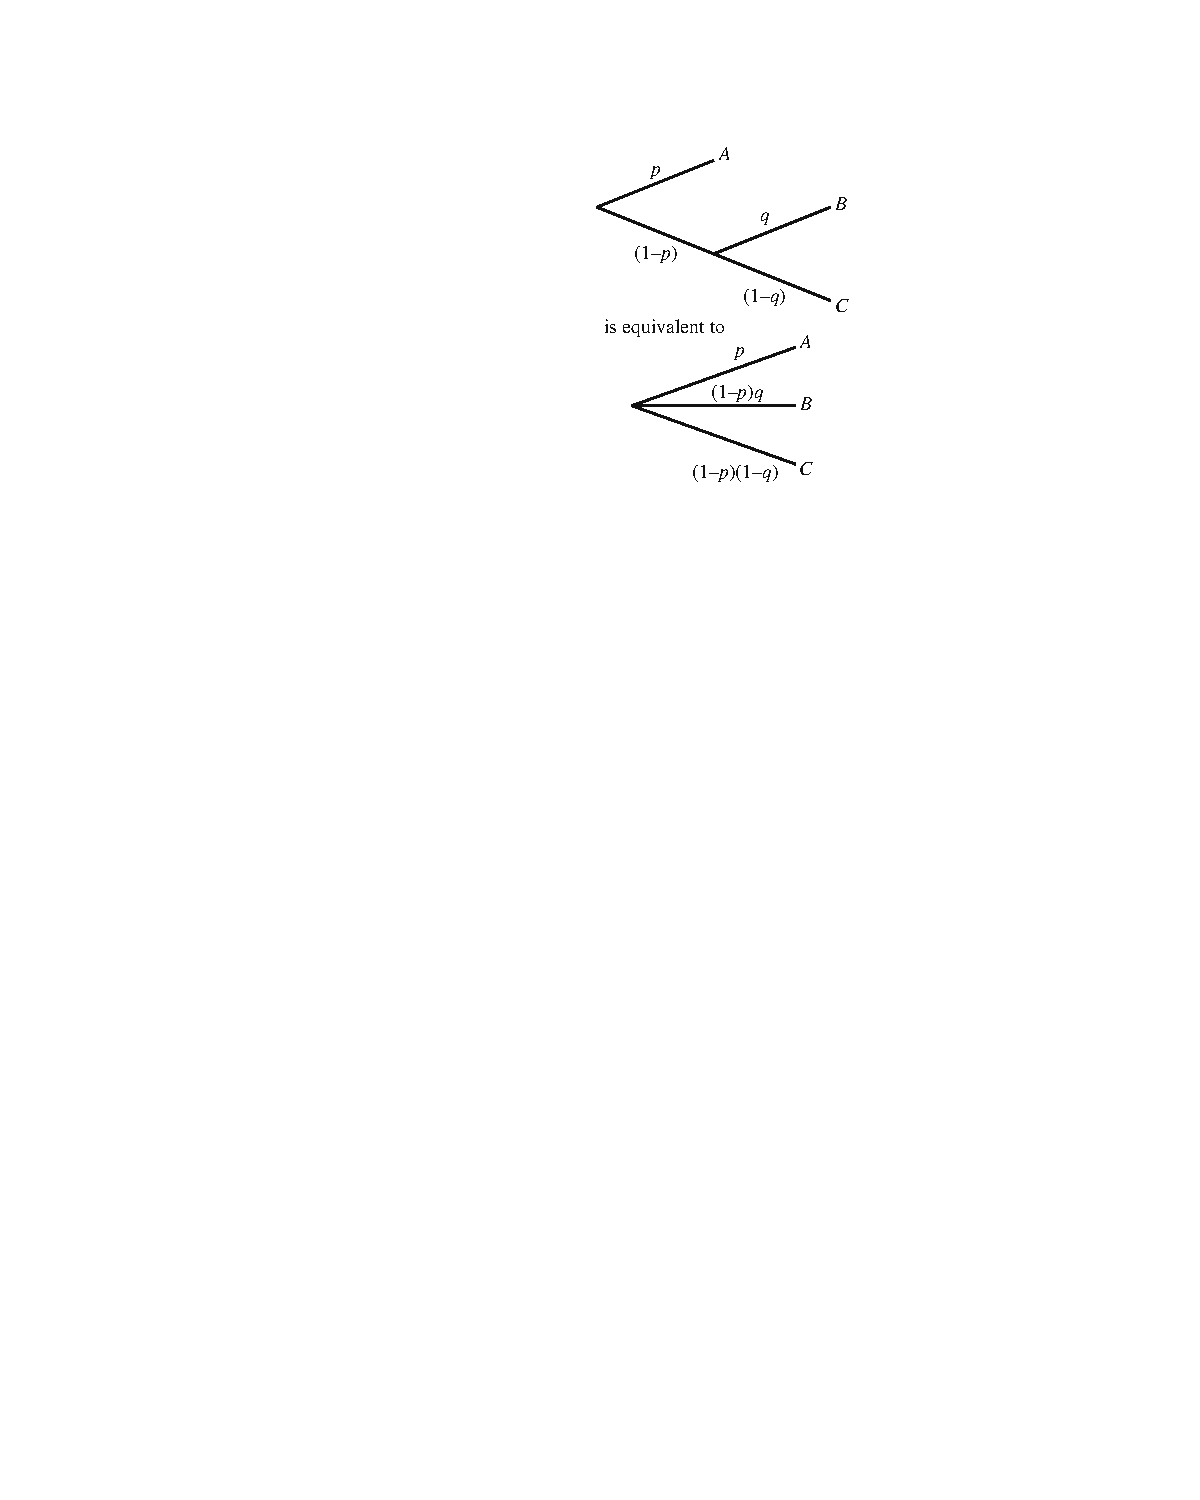
\includegraphics[alt={aima fig 16_01_b decomposability axiom},width=0.75\linewidth]{aima-fig-16_01_b-decomposability-axiom.pdf}
\section{Nontransitive Preferences}
\label{sec:orga3778c5}

Suppose an agent held the following preferences for freely exchangeable goods: \(A \succ B \succ C \succ A\).

This agent would be willing, e.g., to exchange \(B\) plus \$.01 for \(A\), and so on.  But the nontransitivity of the agent's preferences could lead to a cycle that ends in complete financial depletion:



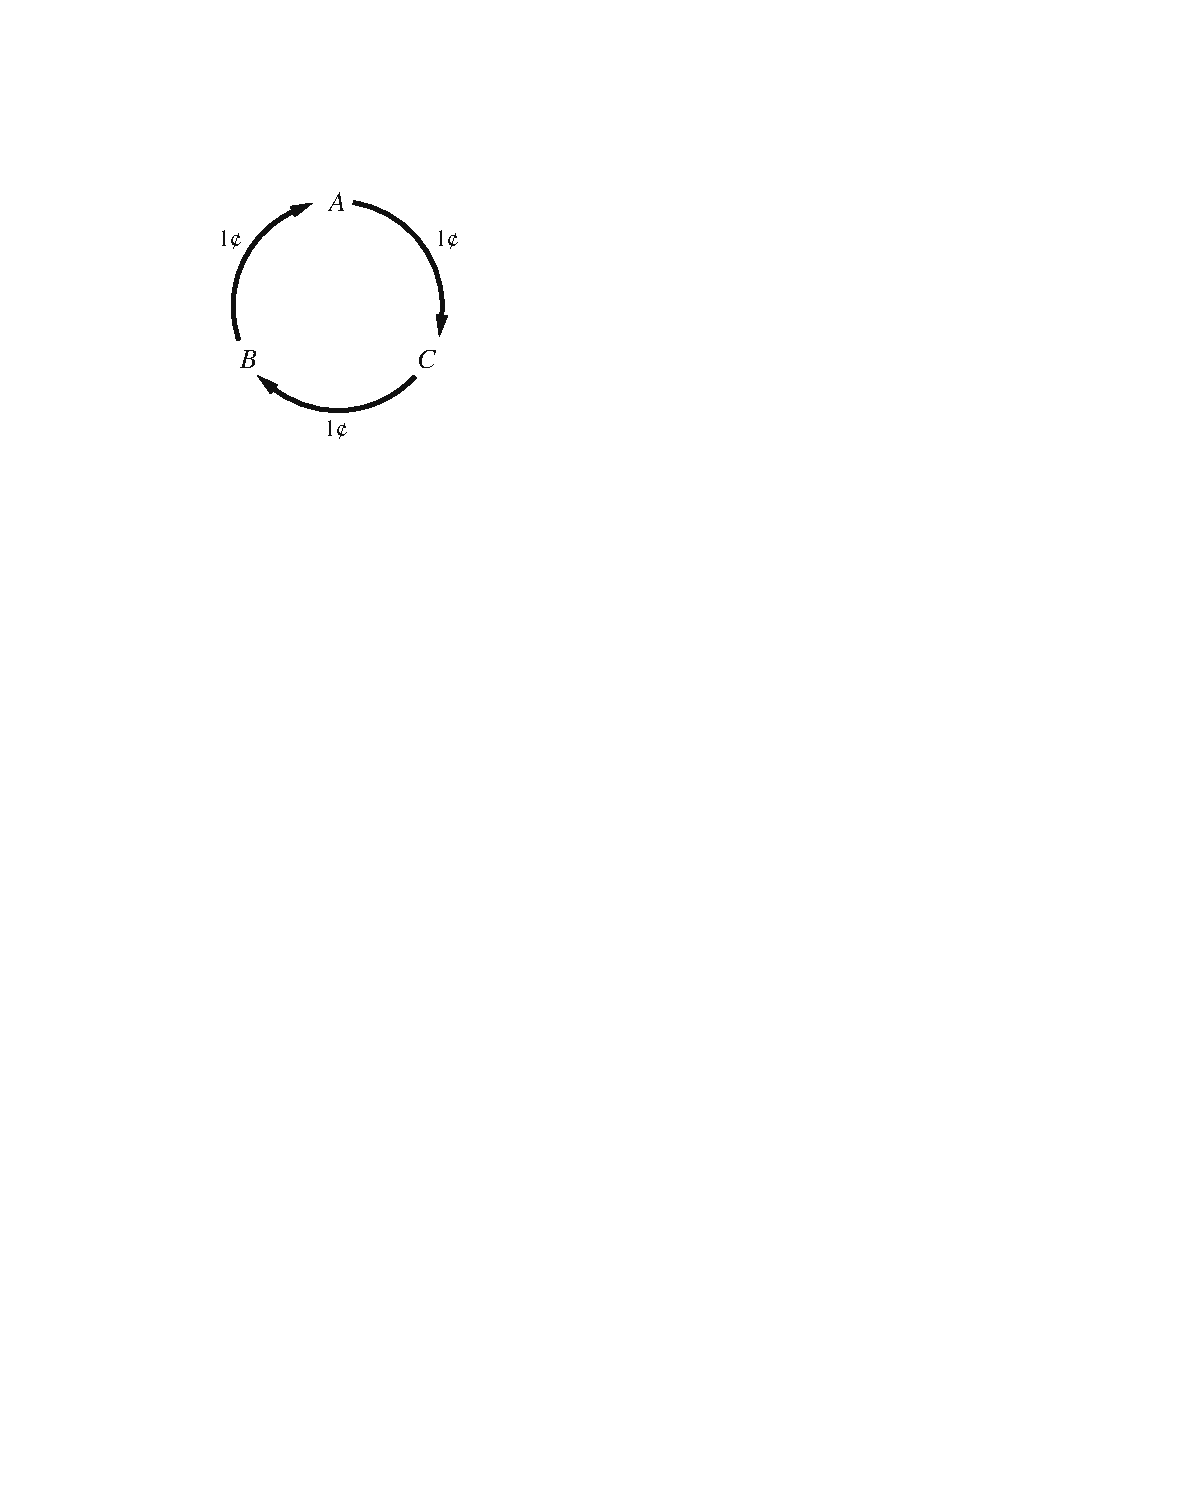
\includegraphics[alt={aima fig 16_01_a nontransitive preferences},width=0.75\linewidth]{aima-fig-16_01_a-nontransitive-preferences.pdf}



The axioms of utility theory are rational because violating them leads to bad outcomes.
\section{From Rational Preferences to Untilities}
\label{sec:org64a67f4}

\begin{itemize}
\item \textbf{Existence of Utility Function}: If an agent’s preferences obey the axioms of utility, then there exists a function U such that \(U(A) > U(B)\) if and only if \(A\) is preferred to \(B\), and \(U(A) = U(B)\) if and only if the agent is indifferent between \(A\) and \(B\). That is,

\begin{itemize}
\item \(U(A) > U(B) \iff A \succ B\) and \(U(A) = U(B) \iff A \sim B\).
\end{itemize}

\item \textbf{Expected Utility of a Lottery}: The utility of a lottery is the sum of the probability of each outcome times the utility of that outcome.

\begin{itemize}
\item \(U([p_1,S_1; \dots ; p_n,S_n]) = \sum_i p_i U(S_i)\).
\end{itemize}
\end{itemize}

Utility functions create relative scales, not absolute scales.  For example, if we apply a positive affine transformation:

\begin{equation*}
U'(S) = aU(S) + b \tag{16.2}
\end{equation*}

Then \(U'\) and \(U\) are effectively equivalent because they lead to the same decisions.

So \(U(S)\) is a \textbf{value function} or \textbf{ordinal utility function}, in which an agent needs only a preference ranking on states -- the numbers don’t matter.
\section{Utility Functions}
\label{sec:orgf32ebfd}

A utility functions

\begin{itemize}
\item map from lotteries to real numbers, and
\item obey the axioms of utility theory.
\end{itemize}

Otherwise, they are arbitrary.

\begin{itemize}
\item I might prefer pepperoni pizza to pineapple, another might prefer the reverse.
\item Decisions based on either preference ordering, as long as it follows the two properties above, are rational.
\end{itemize}

To build a decision support system for humans we must try to infer the human's utility function, a process called \textbf{preference elicitation}.
\section{Utility Scales and Preference Elicitation}
\label{sec:org7134283}

There is no absolute scale for utilities, but we can establish some scale.  Let

\begin{itemize}
\item \(U(S) = u_{\top}\) be the best possible prize,
\item \(U(S) = u_{\bot}\) be the worst possible catastrophe, and
\item use a \textbf{normalized utility scale} in which \(u_{\bot} = 0\) and \(u_{\top} = 1\).
\end{itemize}

Then preference elicitation can proceed by

\begin{itemize}
\item asking the agent to choose between a particular prize \(S\) and a \textbf{standard lottery} \([p, u_{\top}; (1-p), u_{bot}]\), and
\item adjusting the probability \(p\) until the agent is indifferent between \(S\) and the standard lottery.
\end{itemize}

Assuming normalized probabilities, the utility of \(S\) is then given by \(p\).  We repeat this process for every \(S\) to get the full utility function.

Example:
\section{The "Value" of Human Life}
\label{sec:orge9970f4}




\begin{itemize}
\item Asbestos in schools paradox.

\item US govt agencies like FDA and EPA use the \textbf{value of a statistical life} to determine the costs and benefits of regulations.  In 2019 this was \$10M.

\item A \textbf{micromort} is a one in a million chance of death.

\begin{itemize}
\item Say driving a car for 230 miles incurs a risk of one micromort.
\item If you drive 92,000 miles that's 400 micromorts.
\item If you're willing to pay \$12,000 more for a car that halves your risk of death, then a micromort has a value of \$60 to you.
\end{itemize}

\item \textbf{QALY} is quality-adjusted life year. Patients are willing to accept a shorter life expectancy to avoid a disability.
\end{itemize}




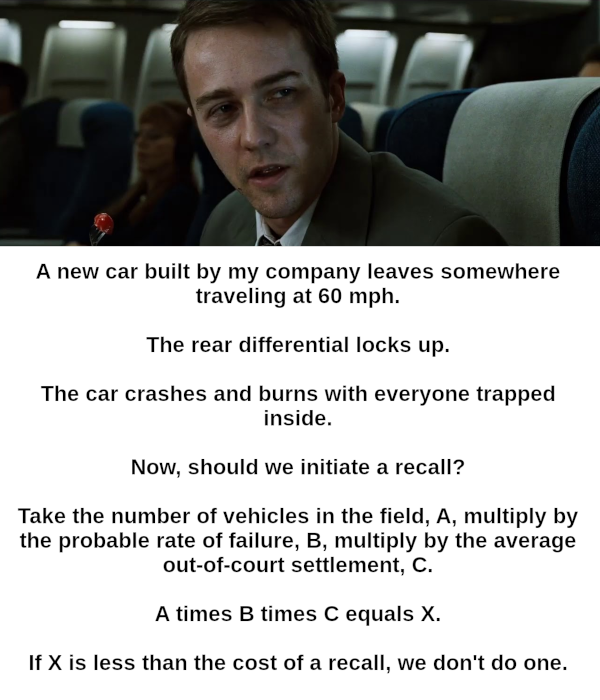
\includegraphics[alt={fight club formula meme},height=3.2in]{fight-club-formula-meme.png}
\section{The Utility of Money}
\label{sec:orgb5ce3e7}

Money is an obvious candidate for a utility measure.

\begin{itemize}
\item Most agents exhibit a \textbf{monotonic preference} for more money.
\item However, money is not necessarily a utility function because it says nothing about preferences between \textbf{lotteries} involving money.

\begin{itemize}
\item Example: Choose between \$1,000,000 and a 50\% chance for \$2,500,000.
\item The \textbf{expected monetary value} (EMV) of the gamble is \$.5 ($\backslash$$0) + .5 ($\backslash$$2,500,000) = $\backslash$\(1,250,000\)
\end{itemize}
\end{itemize}

Key idea: value of money not directly proportional to utility.

\begin{itemize}
\item Let \(k\) be current wealth and \(S_n\) be the state of posessing total wealth of \(n\) dollars.
\end{itemize}

\begin{align*}
EU(Accept)  &= \frac{1}{2} U (S_k) + \frac{1}{2} U (S_{k+2,500,000}) \\
eu(Decline) &= U(S_{k+1,000,000})
\end{align*}

Now say \(U((S_k) = 5\), \(U(S_{k+2,500,000})\) = 9\$, and \(U(S_{k+1,000,000} = 8\).  Then

\begin{itemize}
\item \(EU(Accept) = 7\)
\item \(EU(Decline) = 8\)
\end{itemize}

"Utility of your first million is higher than your second."  A billionaire would likely have a locally linear utility function over such small amounts, so would accept the gamble.
\section{Utility of Money Example}
\label{sec:org7d06069}


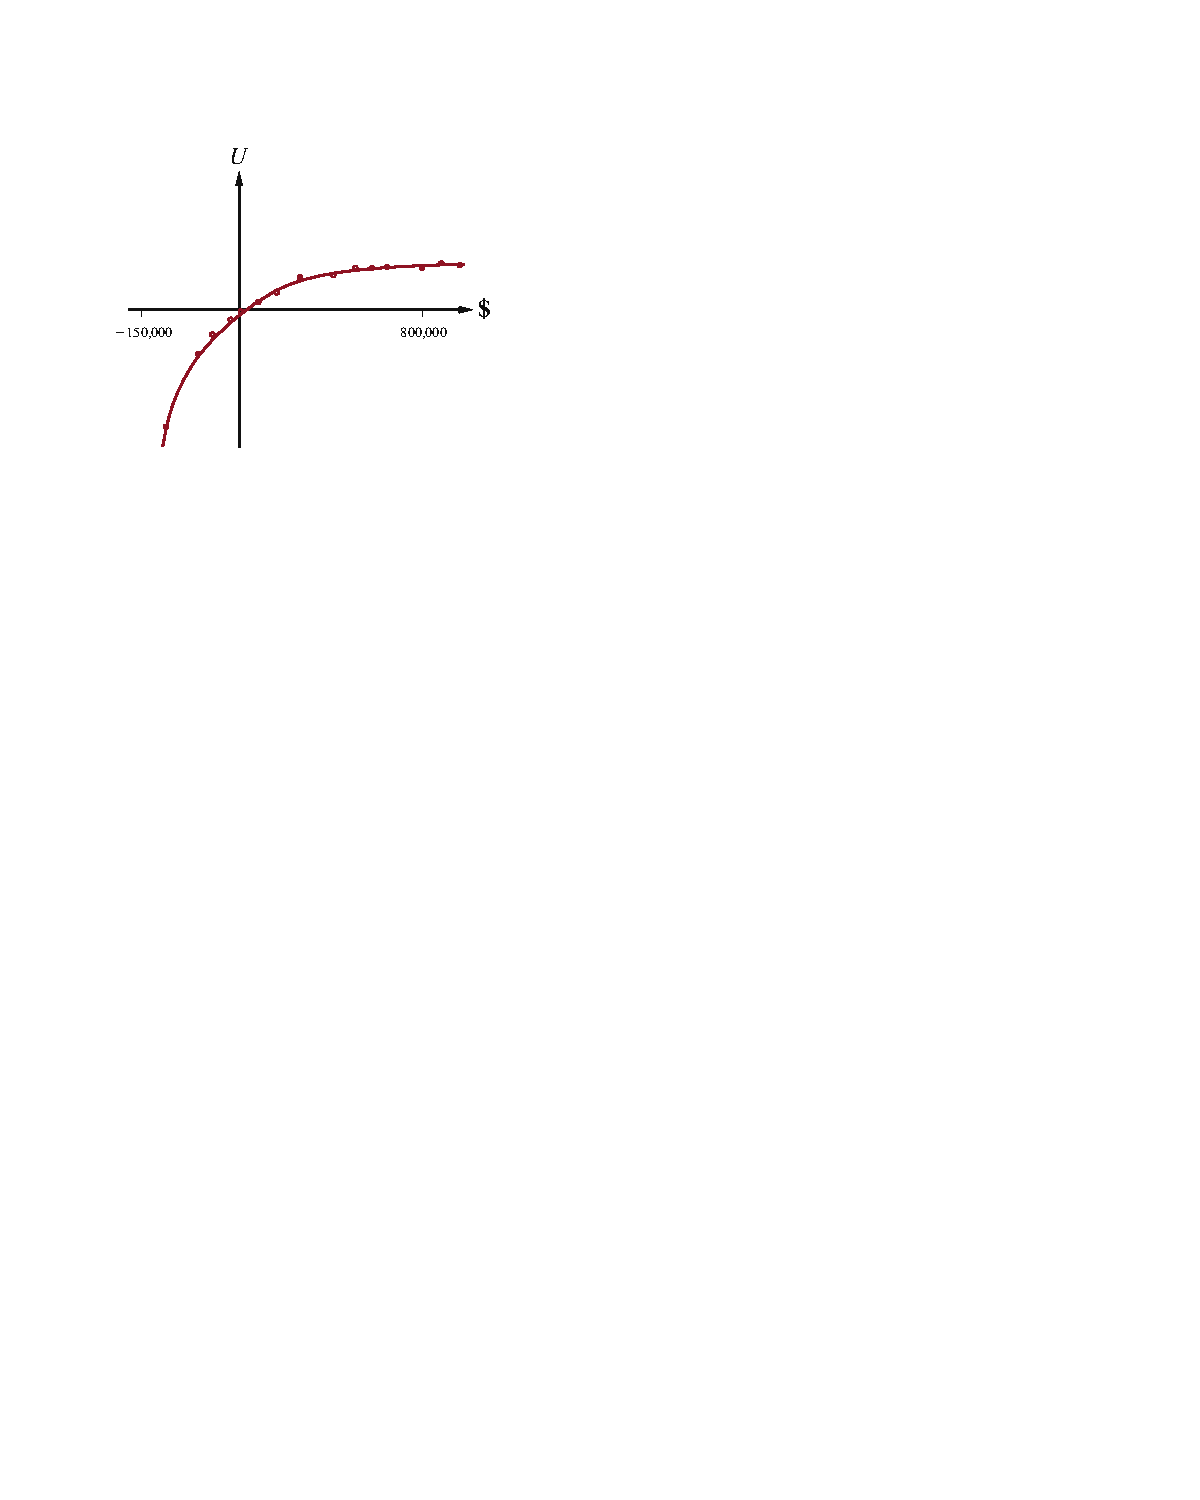
\includegraphics[alt={aima fig 16_02_a utility of money mr beard},width=0.75\linewidth]{aima-fig-16_02_a-utility-of-money-mr-beard.pdf}
\section{Utility of Money in General}
\label{sec:org6db6159}


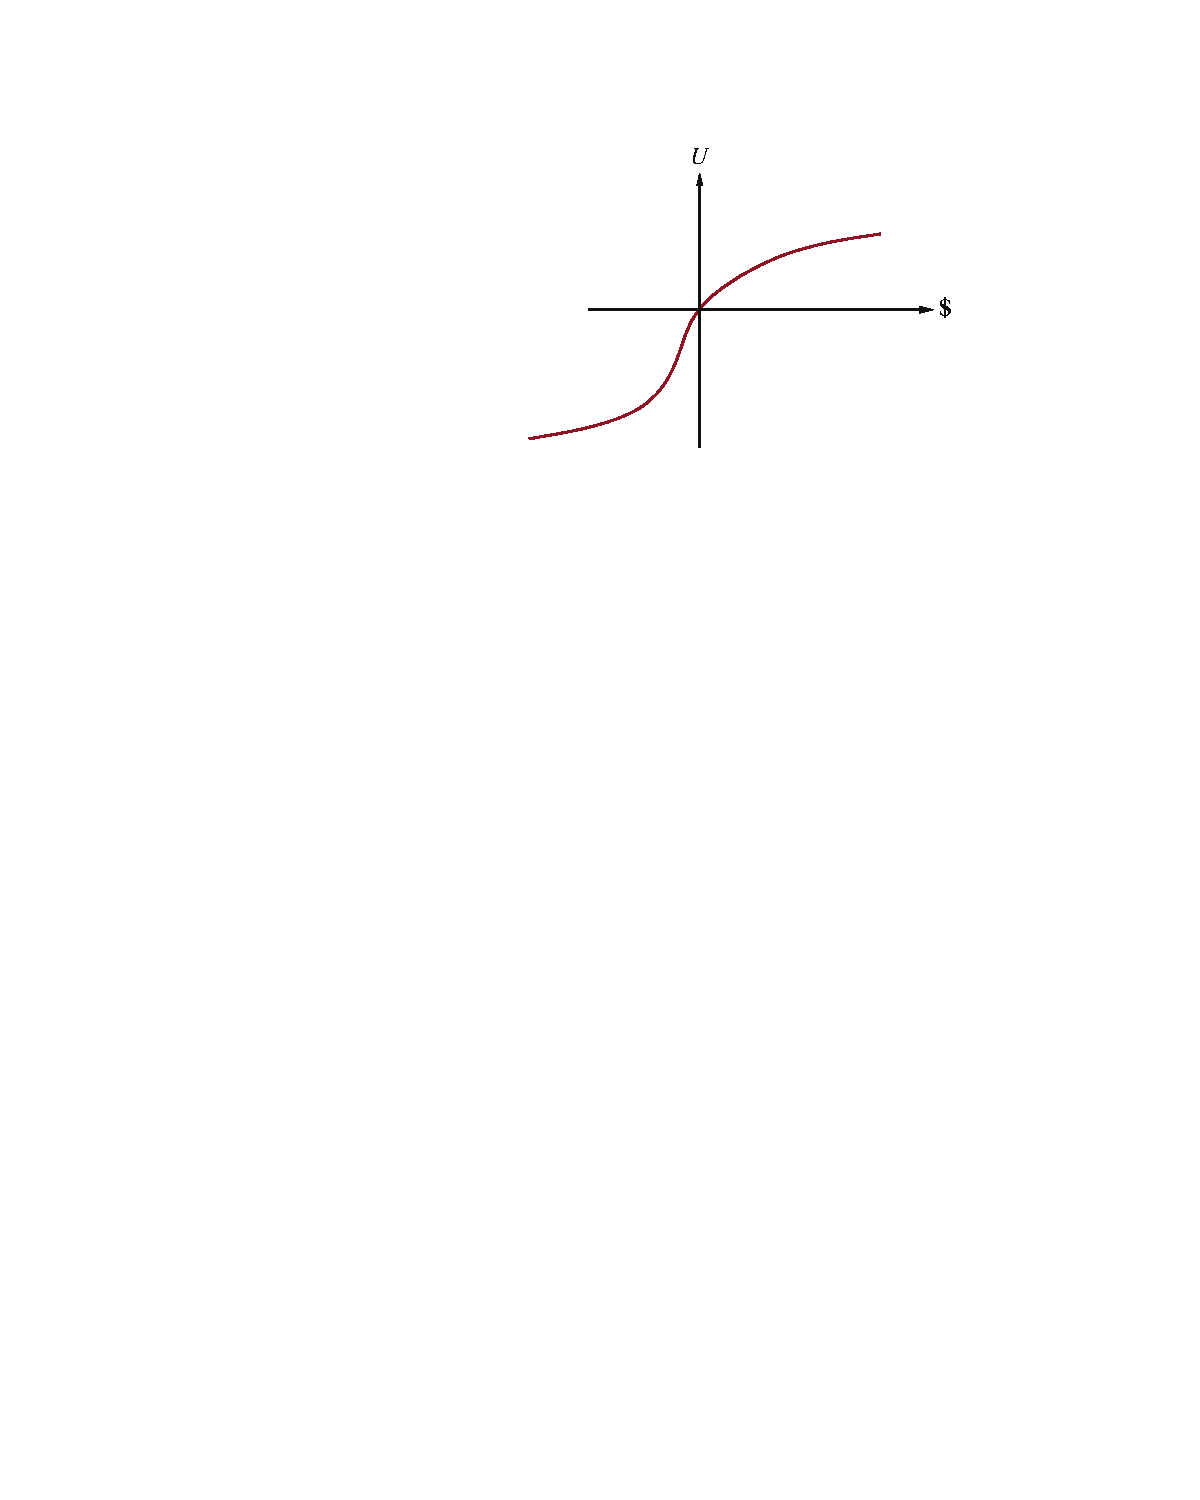
\includegraphics[alt={aima fig 16_02_b utility of money full range},width=0.75\linewidth]{aima-fig-16_02_b-utility-of-money-full-range.pdf}
\section{The Optimzer's Curse}
\label{sec:org1b12a14}

The greater the number of choices, the more biased your estimates are because you always pick "optimal" action.


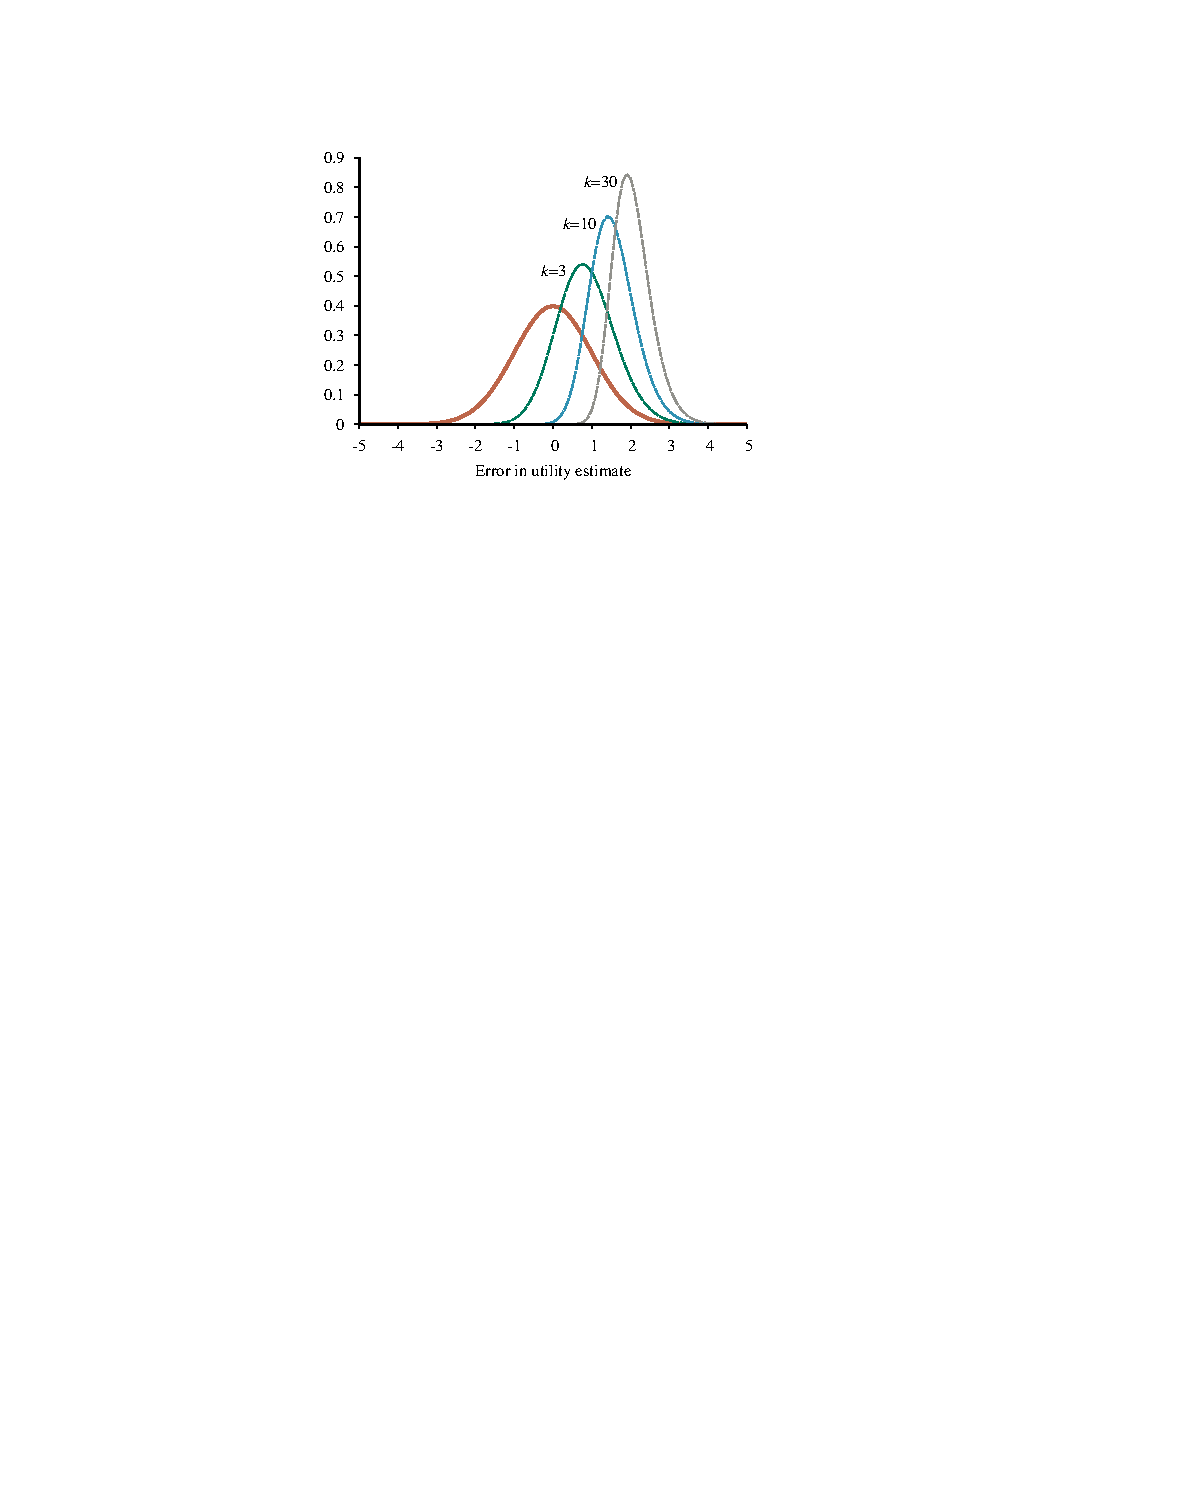
\includegraphics[alt={aima fig 16_03 optimism error},width=0.75\linewidth]{aima-fig-16_03-optimism-error.pdf}
\section{Human Judgement and Irrationality}
\label{sec:org44f1fac}




\begin{itemize}
\item Decision theory is a \textbf{normative theory} -- how people \textbf{should} act.
\item Actualy behavior is described by a \textbf{descriptive theory}.
\end{itemize}

Humans aren't "rational." (Ariely, 2009)

Allais Paradox: people don't act in accordance with utility theory.

Common errors in thinking:

\begin{itemize}
\item Ambiguity aversion
\item Framing effect
\item Anchoring effect
\end{itemize}









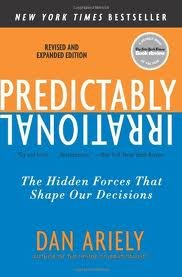
\includegraphics[alt={predictably irrational book},height=1.6in]{predictably-irrational-book.jpg}



\includegraphics[alt={dan ariely},height=1.6in]{dan-ariely.png}






{[}\textsuperscript{DanAriely}]: \url{https://web.mit.edu/ariely/www/}
\section{Multiattribute Utility Functions}
\label{sec:orga026edd}

Let the attributes be \(\bm{X} = X_1, \dots, X_n\) and the vector \(\bm{x} = \langle x_1, \dots, x_n \rangle\) be a complete set of variable values.

\begin{itemize}
\item Each \(x_i\), whether continuous or discrete, must be from a totally ordered set.
\item Not required, but better if higher values mean higher utilities, i.e., each \(x_i\) monotonically increases.

\begin{itemize}
\item \(-d\) deaths better than \(d\), assuming you prefer fewer deaths.
\item Measures with a peak that falls off in either direction could be split.  E.g., instead of temperature \(t\) with peak at 70, have:

\begin{itemize}
\item Warmth, \(w = \min (0, t - 70)\) with max value of 0.
\item Coolness, \(c = \min (0, 70 - t)\) with max value of 0.
\end{itemize}
\end{itemize}
\end{itemize}

Two ways to deal with multiattribute utility funcitons:

\begin{itemize}
\item Keep attributes separate.
\item Combine attributes into a single utility value.
\end{itemize}
\section{Airport Siting Problem}
\label{sec:org40daa52}

Attributes of airport siting problem (where to locate an aiport):

\begin{itemize}
\item \(X_1\): Throughput, measured by the number of flights per day;
\item \(X_2\): Safety, measured by minus the expected number of deaths per year;
\item \(X_3\): Quietness, measured by minus the number of people living under the flight paths;
\item \(X_4\): Frugality, measured by the negative cost of construction.
\end{itemize}
\section{Strict Dominance}
\label{sec:org531aaba}




Given two airport sites \(S_1 = \langle x_1^{(1)}, x_2^{(1)}, x_3^{(1)}, x_4^{(1)} \rangle\) and \(S_2 = \langle x_1^{(2)}, x_2^{(2)}, x_3^{(2)}, x_4^{(2)} \rangle\):


\begin{itemize}
\item If \(x_i^2 < x_i^1, \forall i\), then \(S_1\) \textbf{strictly dominates} \(S_2\).
\item Helpful for eliminating choices, rarely sufficient to find a unique best choice.
\end{itemize}





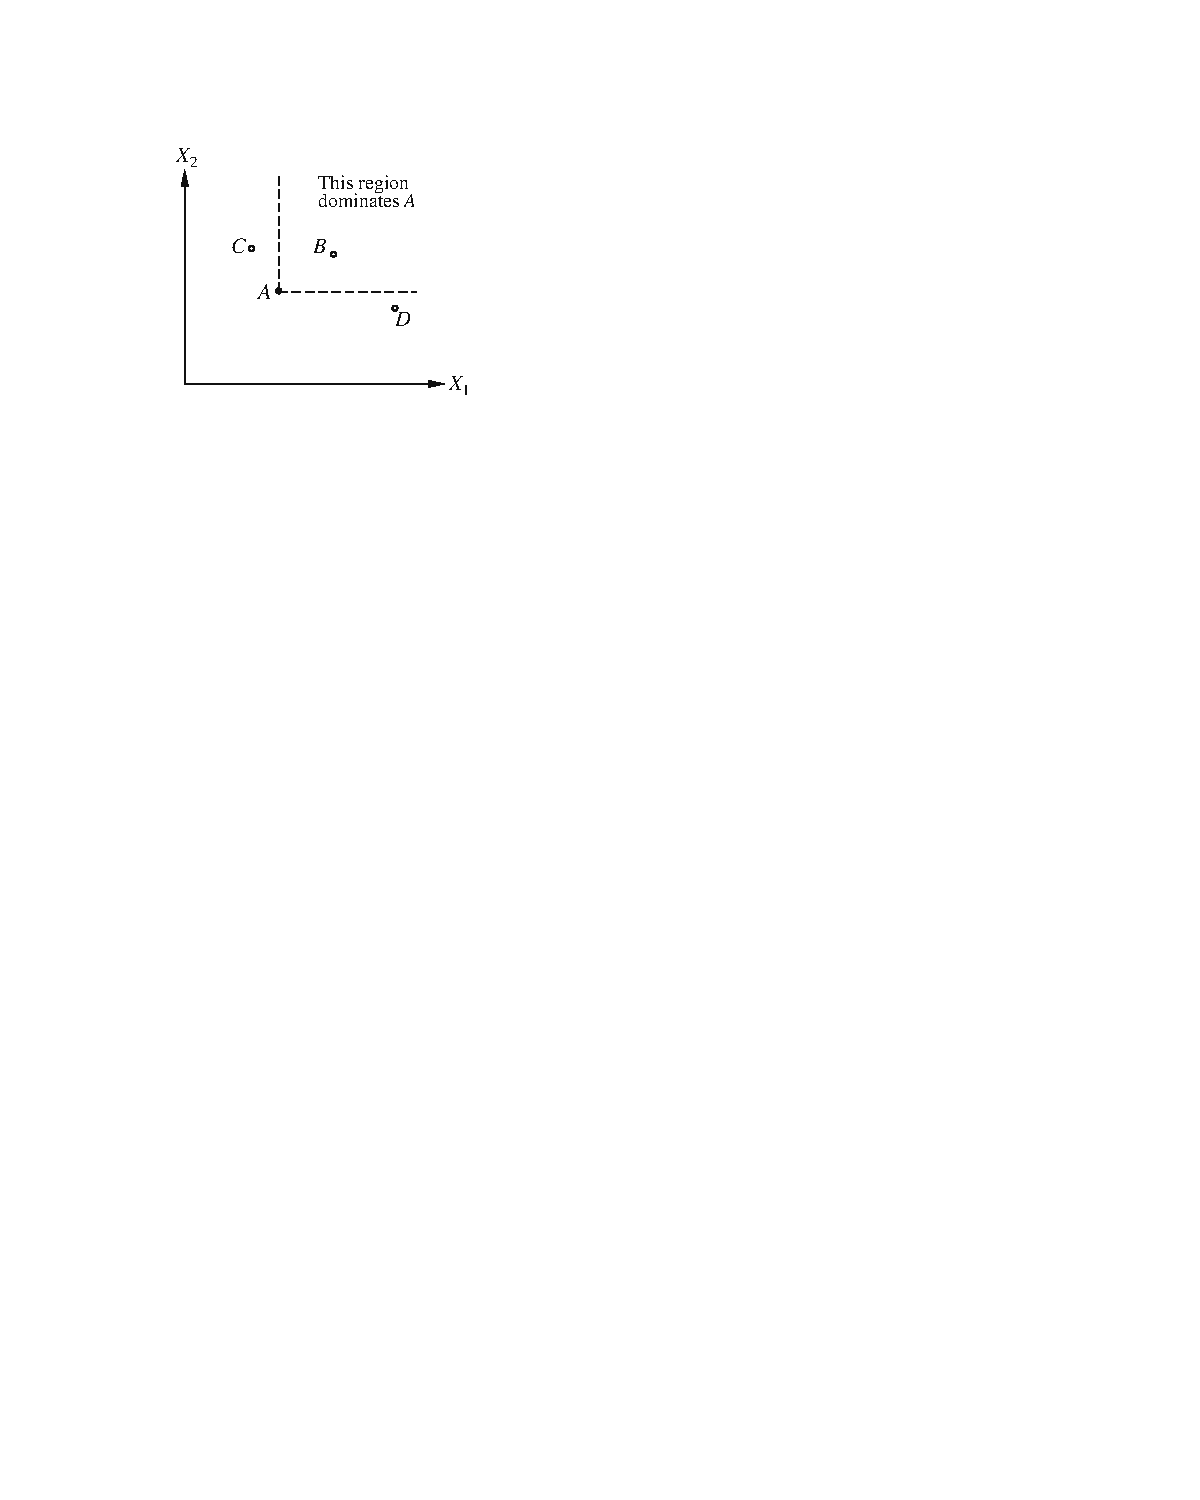
\includegraphics[alt={aima fig 16_04_a dominance deterministic},width=0.75\linewidth]{aima-fig-16_04_a-dominance-deterministic.pdf}
\section{Preference Structure}
\label{sec:orgd86d305}

Specifying complete utility function \(U(x_1, \dots, x_n)\) requires \(d^n\) values in the worst case.  Avoid this complexity by encoding some structure of preferences into \textbf{representation theorems}:

\begin{equation*}
U(x_1, \dots, x_n) = F\left[f_1(x_1), \dots, f_n(x_n) \right]
\end{equation*}

Where

\begin{itemize}
\item \(F\) is a simple function (like addition), and
\item each \(f_i\) converts utility attributes into a common measure.
\end{itemize}

Example: Each \(x_i\) is an amount of money in an abitrary currency like Euros or Rupees, and each \(f_i\) converts the amount into USD.
\section{Deterministic Preferences}
\label{sec:orgee1de75}

Most common regularity in deterministic preferences is \textbf{preference independence}:

\begin{itemize}
\item Two attributes \(X_1\) and \(X_2\) are preferentially independent of a third attribute \(X_3\) if the preference between outcomes \(\langle x_1,x_2,x_3 \rangle\) and \(\langle x'_1,x'_2,x_3 \rangle\)
\end{itemize}
does not depend on the particular value \(x_3\) for attribute \(X_3\).

Airport siting example: let \(X_1 = Quietness\), \(X_2 = Frugality\), \(X_1 = Safety\), with

\begin{itemize}
\item \(x_1\) = 70,000 people living under flight path,
\item \(X_2\) = \$3.7 Billion constuction cost, and
\item \(x_3\) = 0.006 deaths per billion passenger miles.
\end{itemize}

If we prefer \(\langle 20,000, 4B, 0.006 \rangle\), then this preference would hold for any \(x_3\).
\section{Mutial Preference Independence}
\label{sec:org150fcab}

\textbf{Mutual prefence independence} (MPI) means that preference for each attribute has no effect on preference for other attributes.  When this holds, the agent's preferences can be represnented by a value function of the form:

\begin{equation*}
V(x_1,, \dots, x_n) = \sum_i V_i(x_i)
\end{equation*}

For example, we could assume MPI for the airport siting problem and use the value funciton:

\begin{equation*}
V(quietness, frugality, safety) = quietness \times 10^4 + frugality + safety \times 10^{12}
\end{equation*}

This is an example of an \textbf{additive value function}.  Even when MPI doesn't hold, can be a useful simplifying assumption.
\section{Non-MPI Example}
\label{sec:orgea879ba}




You're purchasing some hunting dogs, some chickens, and some cages for the chickens.

\begin{itemize}
\item The hunting dogs are very valuable, but will eat uncaged chickens.
\item So you need enough cages for the chickens.
\end{itemize}

Hence, the tradeoff between dogs and chickens depends strongly on the number of cages, and MPI is violated.




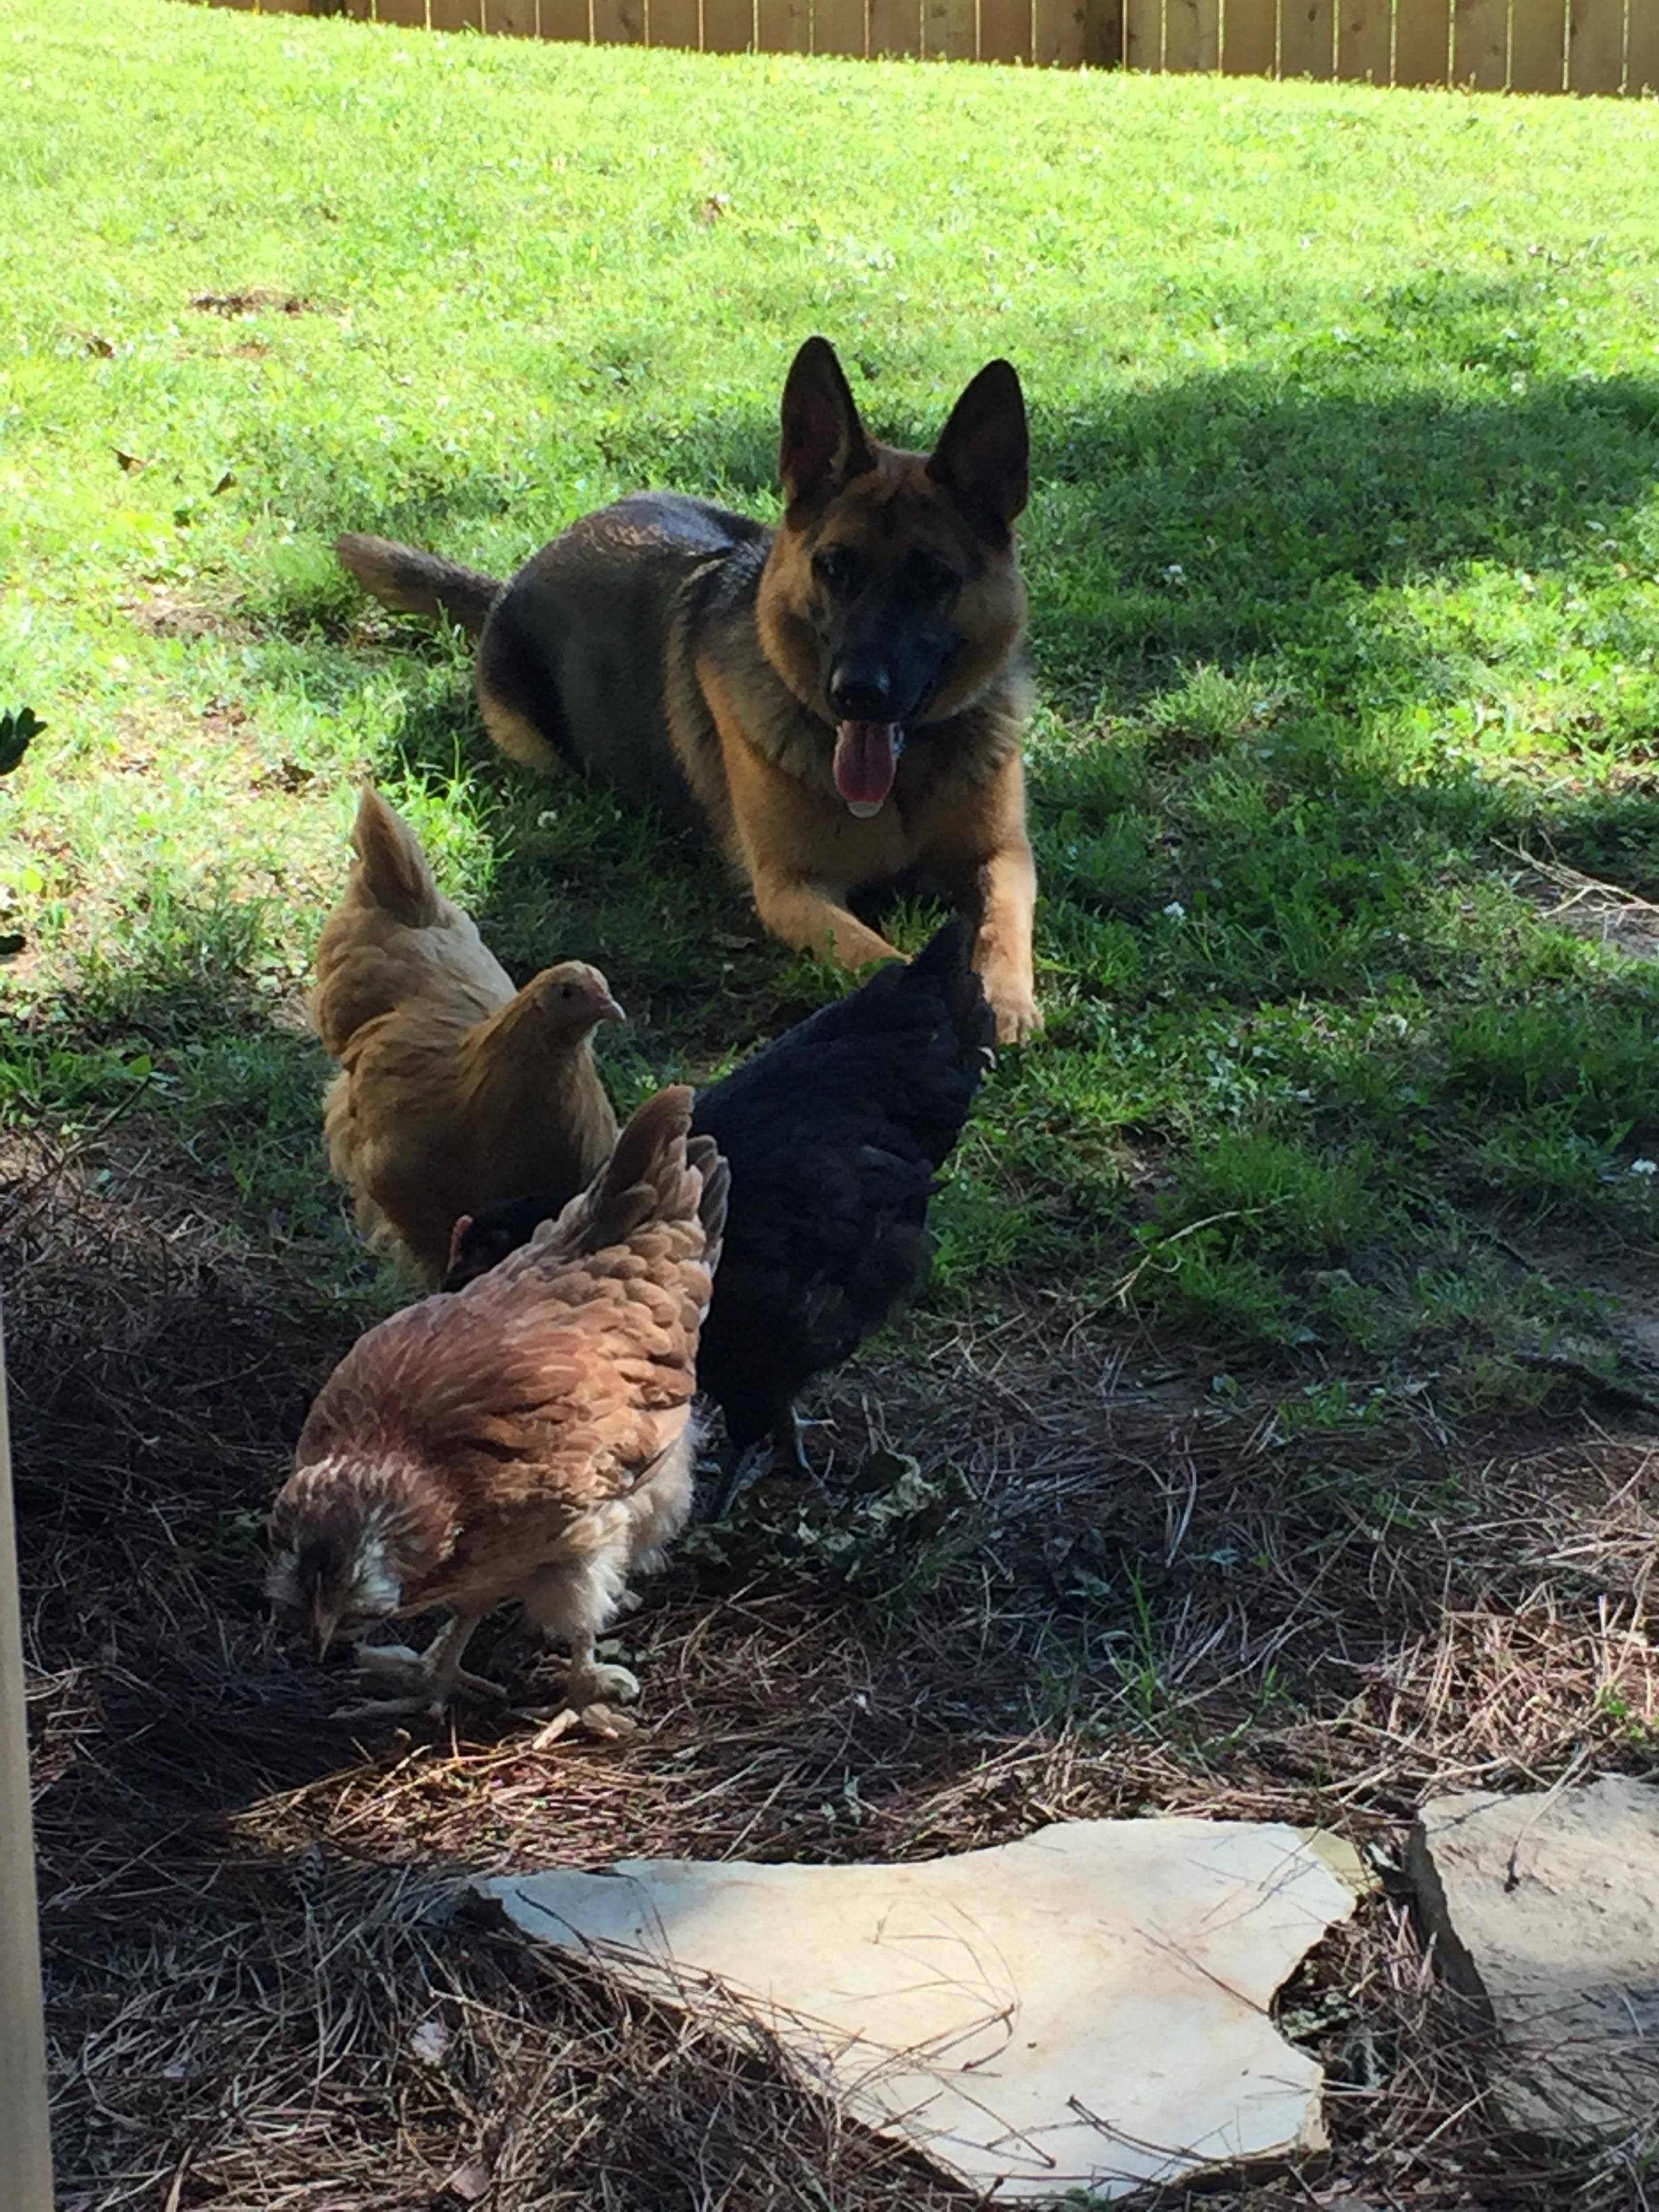
\includegraphics[alt={shepherd chickens},height=3.0in]{shepherd-chickens.jpg}





{[}\textsuperscript{ShepherdChickens}]: \url{https://www.reddit.com/r/germanshepherds/comments/p4sou1/our\_girl\_reyna\_watches\_her\_flock\_8\_of\_backyard/}
\section{Syntax of Decision Networks}
\label{sec:org171f4e8}




\begin{itemize}
\item Chance nodes (ovals) represent random variables, like in Bayesian networks.

\begin{itemize}
\item Agent could be uncertain about the construction cost, level of air traffic, potential for litigation, and Safety, Quietness, Frugality variables, each of which also depends on the site chosen.
\item Each chance node has a conditional distribution indexed by state of its parent nodes.
\item Parent nodes can include decision nodes and chance nodes.
\item Each current-state chance node could be part of a large Bayesian network for assessing construction costs, air traffic levels, or litigation potentials.
\end{itemize}
\end{itemize}

\vspace{.1in}





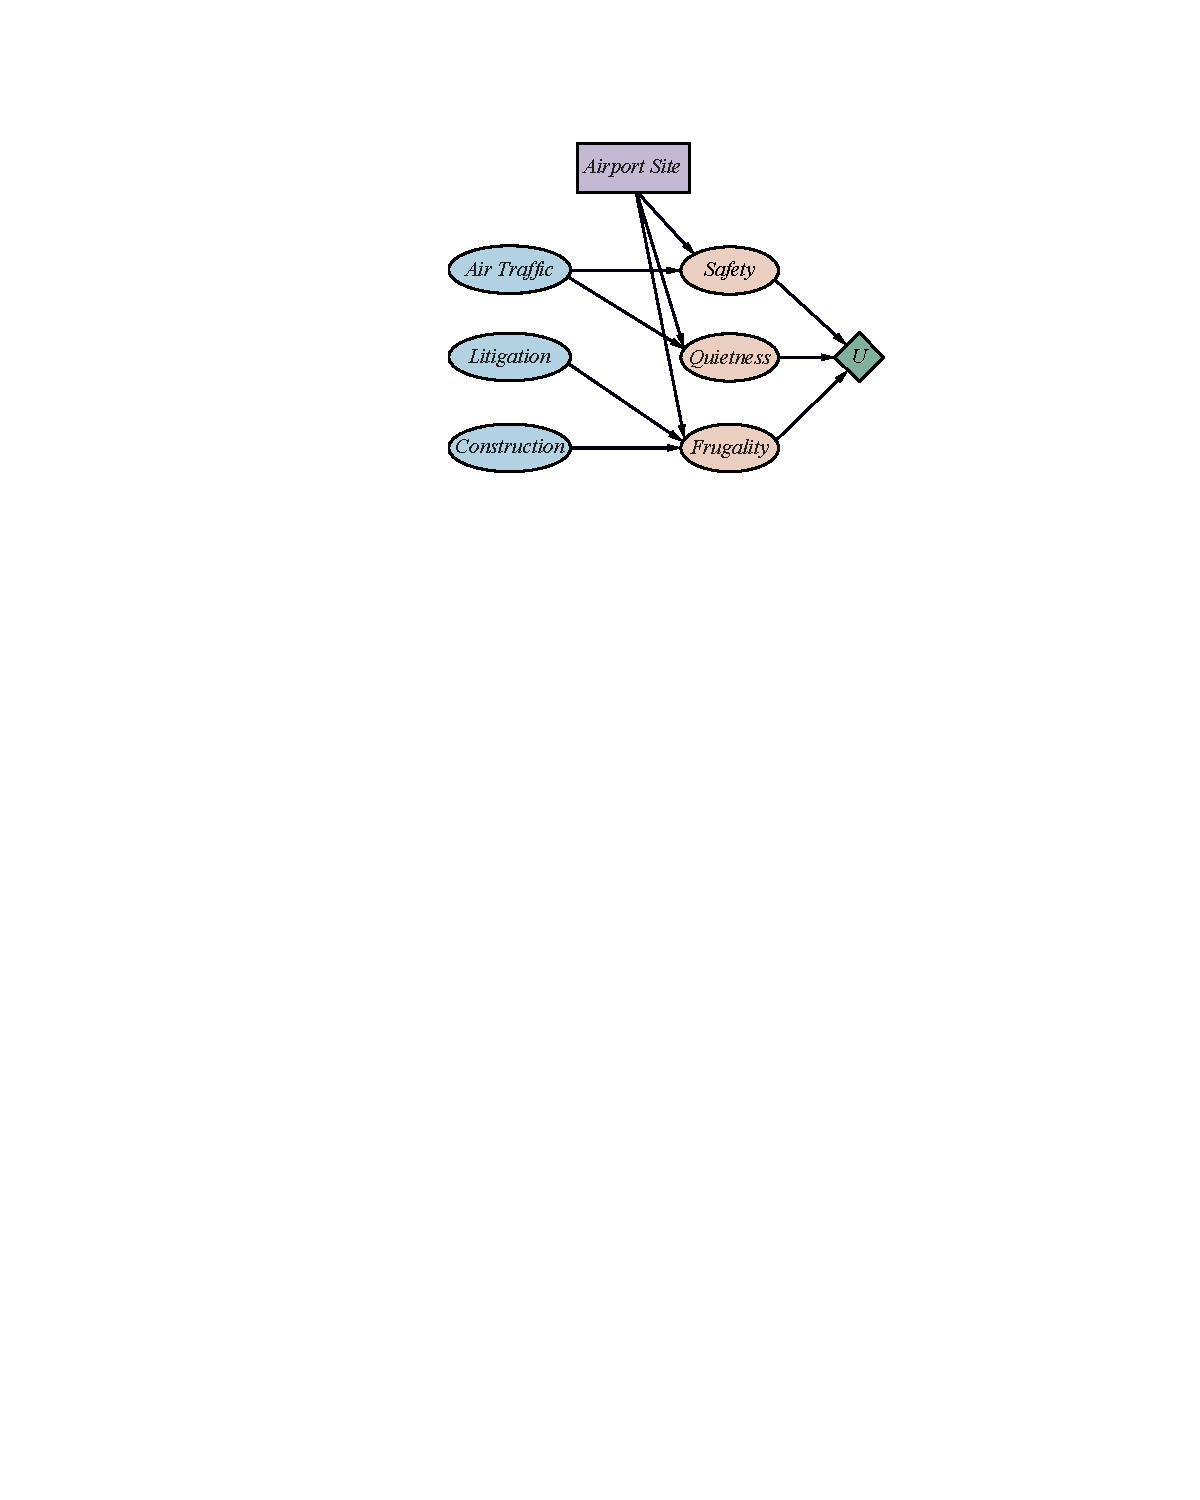
\includegraphics[alt={aima fig 16_06 decision network airport siting},width=0.75\linewidth]{aima-fig-16_06-decision-network-airport-siting.pdf}
\end{document}
